\documentclass[10pt,pdf,hyperref={unicode}]{beamer}
\usepackage[utf8]{inputenc}
\usepackage[russian]{babel}
\usepackage{graphicx}
\usetheme{Madrid}

\usenavigationsymbolstemplate{}
\setbeamertemplate{footline}[frame number]

\begin{document}

    \title[GoogleNotifier]{SPbAU Google Notifier}
    \subtitle{НИР, весна 2014}
    \author{Богдан Бугаев, Тимур Тураев \\ Руководитель: Евгений Краско}
    \date{26 мая 2014 г.}
    \institute{Академический университет}
    
    \titlegraphic{
\includegraphics[scale=0.25]{qrcode.png}}

    \begin{frame}
		\titlepage
	\end{frame}
    
    \begin{frame}\frametitle{О проекте}
        \begin{itemize}
        	\item	Google-документы часто изменяются
	       	\item	Бывает важно быстро узнать, что изменился тот или иной документ
	       	\pause
            \item	Google позволяет отследить изменения одного конкретного документа
            \pause
            \item	На эти изменения нужно подписываться вручную
            \pause            
            \item	Это не очень удобно, когда документов много
            \pause            
            \item	Хочется автоматически следить за всеми документами разом
            \pause            
            \item	С помощью настольного приложения
        \end{itemize}
    \end{frame}    
    
    \begin{frame}\frametitle{Архитектура}
    	\begin{figure}[ht] 
            \begin{minipage}[b]{0.5\linewidth}
                \centering
                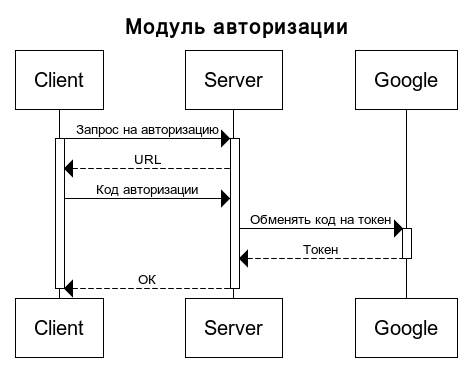
\includegraphics[scale=0.25]{auth.png} 
            \end{minipage}%%
            \begin{minipage}[b]{0.5\linewidth}
                \centering
	            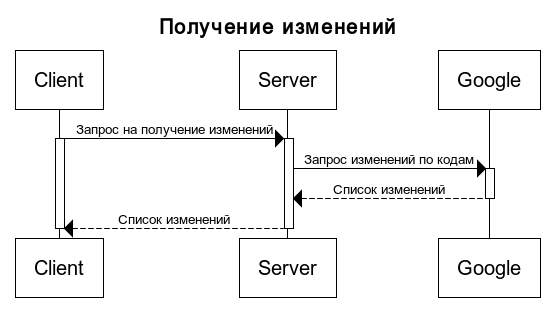
\includegraphics[scale=0.25]{changes.png} 
            \end{minipage}
            \begin{minipage}[b]{0.5\linewidth}
    	        \centering
                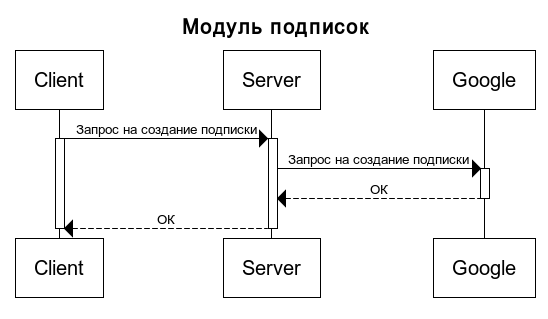
\includegraphics[scale=0.25]{subscription.png} 
            \end{minipage}%%
            \begin{minipage}[b]{0.5\linewidth}
                \centering
                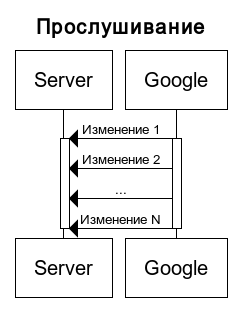
\includegraphics[scale=0.25]{listening.png} 
            \end{minipage} 
        \end{figure}
        \begin{itemize}%[<+->]
            \item	Google позволяет подписаться на все изменения сразу всех документов
            \pause
            \item   Уведомления об изменениях Google посылает на сервер
            \pause
            \item   Клиенты подключаются к нашему серверу, получая все поступившие изменения документов
        \end{itemize}
    \end{frame}

    \begin{frame}\frametitle{Задачи}
        \begin{itemize}%[<+->]
        	\item Серверная часть
	        \begin{itemize}
                \item модуль авторизации
                \item модуль по работе с подписками
                \item модуль обработки приходящих изменений от Google
            \end{itemize}            
            \pause
        	\item Клиентская часть
	        \begin{itemize}
                \item модуль сетевого взаимодействия
                \item модуль GUI
                \item модуль визуализации уведомлений (notifications)
            \end{itemize}                        
        \end{itemize}
    \end{frame}
    
    \begin{frame}\frametitle{Проблемы (серверная часть)}
        \begin{itemize}%[<+->]
	        \item	Хостинг, web-framework
	        \pause
            \begin{itemize}
                \item GAE (Google App Engine)
                \item webApp2 (Python)       
            \end{itemize}
	        \pause
            \item	Ограниченное непродляемое время жизни подписки на изменения
	        \pause
            \begin{itemize}
                \item Сохранение состояние в параметрах сессии
                \item Клиент сам обновляет подписку
            \end{itemize}
	        \pause
            \item	Push-уведомлений с изменениями от Google идут на зарегистрированный сервер и содержат только номер изменения
	        \pause
            \begin{itemize}
                \item Зарегистированный сайт
                \item Сохранение изменений в базу данных
                \item Сервер (по запросу клиента) запрашивает у Google информацию об изменениях по их номеру
            \end{itemize}
        \end{itemize}
    \end{frame}
    
    \begin{frame}\frametitle{Результаты (серверная часть)}
        \begin{itemize}%[<+->]
            \item	Написан веб-сервер, обрабатывающий запросы, поступающие от клиентов            
            \item	Авторизация, аутентификация, сессии, защита cookie
	        \pause
            \item	Модуль подписок (с автообновлением)
            \item	Сохранение информации об изменениях в базу данных
	        \pause
            \item	Фильтры
            \begin{itemize}
                \item Изменения самим собой игнорируются
                \item Не посылаются уведомления, в которых время последнего просмотра документа превышает время последнего изменения.
            \end{itemize}

        \end{itemize}
    \end{frame}
    
    \begin{frame}\frametitle{Проблемы (клиентская часть)}
        \begin{itemize}%[<+->]
            \item Выбор языка и библиотек для разработки. Кроссплатформенность
            \pause
            \begin{itemize}
                \item C++
                \item Qt
            \end{itemize}
            \pause
            \item Извлечение изменений с сервера
            \pause
            \begin{itemize}
                \item опрос с заданной периодичностью (polling)
            \end{itemize}
            \pause
            \item Ограниченное непродляемое время жизни подписки на изменения
            \pause
            \begin{itemize}
                \item клиент переподписывается сам c заданной периодичностью
            \end{itemize}
            \pause
            \item Сохранение состояния программы между запусками
            \pause
            \begin{itemize}
                \item запоминание параметров сессии в настройках приложения \\
                (Linux и OS X --- .ini / Windows --- реестр)
            \end{itemize}
            \pause
            \item Особенности Qt 5 под Ubuntu (Unity)
            \begin{itemize}
                \item использование notify-osd
                \item ждем, пока sni-qt адаптируют под Qt 5
            \end{itemize}
        \end{itemize}
    \end{frame}
    
    \begin{frame}\frametitle{Результаты (клиентская часть)}
        \begin{itemize}%[<+->]
            \item Разработано кроссплатформенное ядро клиента            	
            \begin{itemize}
                \item работа с сетью
                \item простой HTTP-сервер
                \item классы для выполнения основных действий
            \end{itemize}
            \pause
            \item Консольный прототип клиента для тестирования функциональности
            \pause
            \item Клиент с графическим интерфейсом под \\ OS X, Ubuntu, Windows
            \begin{itemize}
                \item общая кроссплатформенная часть
                \item платформозависимая часть --- вывод уведомлений
                \item поддерживает сохранение состояния (авторизация, подписка
                на уведомления) между запусками
            \end{itemize}
        \end{itemize}
    \end{frame}

    \begin{frame}\frametitle{Полученные знания}
        \begin{itemize}%[<+->]
            \item	Изучены основные принципы разработки клиент-серверных приложений
            \begin{itemize}
                \item механизм OAuth2 авторизации
                \item механизм построения и разработки веб-сервисов
            \end{itemize}            
            \item	Изучена связка GoogleAppEngine + webApp2 + Google Database API
            \item	Разработка кроссплатформенных приложений на Qt
        \end{itemize}
    \end{frame}

    \begin{frame}
        \begin{center}
            Спасибо за внимание!
        \end{center}
    \end{frame}

\end{document}
